\chapter{Unity}

Dans cette partie il s'agira finalement de parler du développement du module \texttt{Unity} utilisant la nouvelle plateforme mise en place dont il est question Chapitre~\ref{chap:protoHP}. Ce développement a été la parfaite occasion de tester et mettre à l'épreuve cette dernière et avoir un retour réel sur son utilisabilité.
Il sera discuté, dans un premier temps, des apports, mais aussi des enjeux, de la conception et de la cible du module où il sera rapidement aborder les difficultés rencontrés qu'elles soient liés à \texttt{Unity} ou à la nouvelle plate-forme. 
Dans un second temps, nous nous attarderons sur le développement d'une application avec ce module de façon a évaluer s'il réponds aux besoins et si il il y répond de façon efficace.
Pour finir, nous effectuerons une rapide comparaison entre la version actuelle et la version en développement des kit de développement (\texttt{Unity} et \texttt{Processing}) afin d'avoir une évaluation dans des conditions réelles d'utilisation et peut être des pistes d'améliorations de la version \texttt{Unity}.

\section{Module Unity}

L'objectif du module Unity est de permettre à ses utilisateurs d'exploiter la puissance de Nectar (logicielle et matérielle) de façon totalement intuitive afin qu'ils puissent développer des applications de réalité augmentée spatiale sans jamais avoir besoin de se soucier des problèmes liés à cette technologie comme la problématique de calibration du couple caméra projecteur par exemple.
Pour cela, il a fallut créer, dans Unity, les composants et les comportements cruciaux du système tels que les caméras, les caméras de profondeur, les projecteurs, les utilisateurs, la table, et bien d'autres. En plus de résoudre bon nombre de problèmes pour l'utilisateur, ces composants rendent possible la représentation du monde réel Figure~\ref{fig:unityrealworld}. Cette représentation est très importante car, dans le domaine de la réalité augmentée spatiale, où ce dit monde sert de base aux augmentations et, de ce fait, ne peut pas être négligé, en avoir une représentation virtuelle précise permet aux utilisateurs de concevoir leur application dans le même environnement que celui où elles seront projetées.

\begin{figure}[h]
\centering
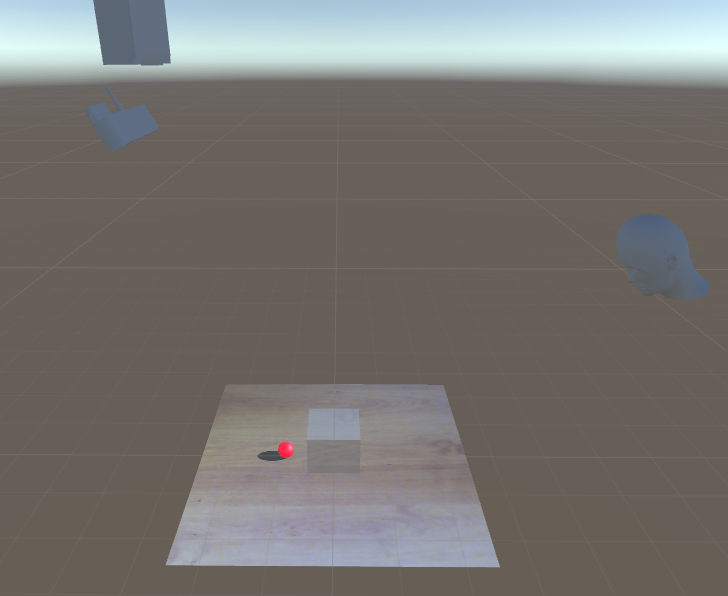
\includegraphics[width=0.65\linewidth]{images/unityscene}
\caption{Représentation du monde dans Unity - A droite, la tête de l'utilisateur, au centre la table, en haut a gauche le couple caméra projecteur.}
\label{fig:unityrealworld}
\end{figure}

Le module Unity possède actuellement deux types de composants:
\begin{itemize}
\item Les composants modélisant les objets matériels du système de projection correspondant aux différents dispositifs d'acquisitions (caméras, projecteurs).
\item Les composants modélisant la partie logiciel correspondant aux divers services de traitement fournis par Nectar.
\end{itemize}

Le fonctionnement d'un composant, peut importe ce qu'il modélise, reste le même. Dans un premier temps, ce dernier créer un client et essai de se connecter à la base de donnée Redis, base dans laquelle tous les services de Nectar, si tant est qu'ils produisent des données, stocke ces dernières. Si Redis n'est pas opérationnel et que la connexion échoue, il s'agit alors d'une erreur critique car cela signifie que Nectar n'a pas non plus pu démarrer ses services. Dans un tel cas, le composant envoie une requête HTTP au serveur Web communiquant avec le gestionnaire de processus Eye, dans le but de redémarrer Redis. Si Redis est toujours déconnecté une message d'erreur critique est remonté à l'utilisateur qui ne pourras utiliser aucun des composants du module jusqu'à ce que Redis soit réparé.

Une fois la connexion avec Redis établie, le composant, encore par le biais d'une requête HTTP, questionne le serveur web sur l'état du service qu'il représente. Par exemple, le composant modélisant la caméra se renseignera sur l'état du service Caméra. Si le service est hors ligne, une requête de démarrage peut être envoyé au serveur web qui la transmet instantanément à Eye afin de rendre opérationnel le service désiré. Si le service désiré n'existe pas un message d'avertissement sur l'indisponibilité de ce dernier est remonté à l'utilisateur qui peut continuer a utiliser les autres composants du module.

Une fois le service démarré où si il était déjà en ligne, le composant peut finalement récupérer les données qu'il produit dans Redis. Pour qu'un composant puisse récupérer ces données, il doit en connaître l'emplacement dans Redis. Redis fonctionnant sur un système de clef/valeur comme expliqué dans la section ~\ref{sec:nectararchi}, la connaissance de la clef est nécessaire c'est pourquoi chaque composant possède un ou plusieurs champ configurable par l'utilisateur pour indiquer les clefs a utiliser pour récupérer les données dans Redis. Par exemple, le composant Caméra qui doit à la fois récupérer les paramètres intrinsèques, extrinsèques et le format des données produite par la caméra possède 3 champ configurable dans Unity pour indiquer leur clef dans Redis.

On peut observer, encadré dans la Figure~\ref{fig:unity:plugin}, les trois points importants du module. 

En vert est représenté la zone où les composants nécessaire à la création d'applications sont ajoutés afin d'en utiliser les fonctionnalités. Ici par exemple, nous utilisons une caméra, un projecteur et une caméra de profondeur rangé dans la partie \emph{hardware}, un point de vue utilisateur \emph{UserPOV (Point Of View)} et différents services comme par exemple le suivi de feuille \emph{Paper Tracker}. Nous avons aussi ajouter a cette scène différents \emph{Renderer} permettant de visualiser les données acquises/générés par les dispositifs d'acquisitions comme la caméra, le projecteur et la caméra de profondeur.

Ensuite, encadré en rouge, on retrouve la zone où il va possible de contrôler l'état des composants et si besoin démarrer les services comme mentionné précédemment. Dans notre exemple, toujours Figure ~\ref{fig:unity:plugin} on observe le script de contrôle du composant projecteur. Ce script permet de spécifier quel type de dispositif on souhaite créer, ici la valeur est \emph{PROJECTOR}, on peut voir l'état interne du composant, ici le composant est dans l'état \emph{WORKING}, ce qui signifie qu'il a réussi à se connecter à  Redis, et qu'il a réussi à récupérer les données dont il avait besoin pour fonctionner, les clefs où sont stockés les dites données a récupérer, et un bouton permettant de démarrer/redémarrer le service en cas d'échec lors de l'initialisation.

Enfin, encadré en bleu, on peut voir la zone où les notifications de tout type (erreur, avertissement, fonctionnement) sont remontés a l'utilisateur pour lui indiquer l'état des services. Chaque notification commence par le nom du composant la générant suivi du message afin de garder une certaine lisibilité.

\begin{figure}[H]
\centering
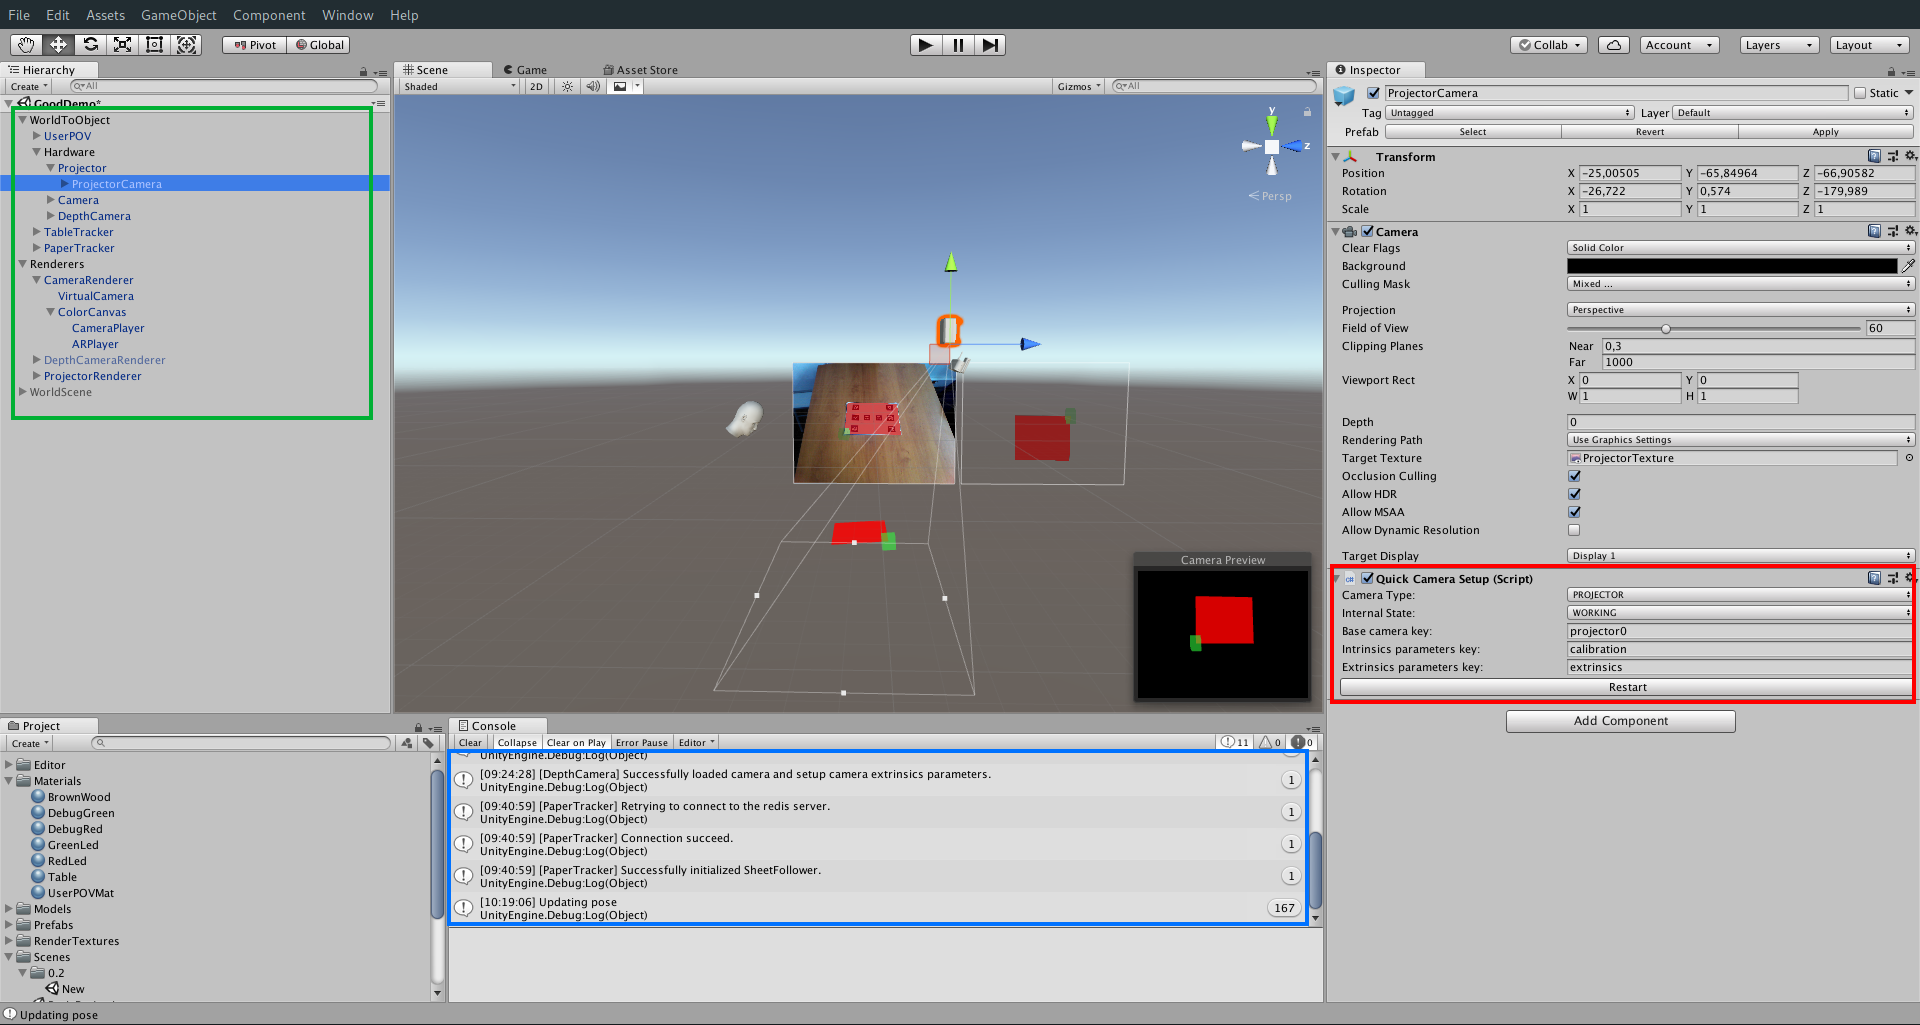
\includegraphics[width=\linewidth]{images/unity-plugin}
\caption{Vue globale du module Unity et de ses différents composants}
\label{fig:unity:plugin}
\end{figure}

Tous les composants et scripts ont été spécialement crée pour s'exécuter directement dans l'éditeur Unity afin de faciliter considérablement le développement pour les utilisateurs. Ainsi il n'est pas nécessaire de construire et exécuté l'application pour pouvoir avoir un retour. Cela permet aussi de gagner en temps précieux et donc d'accélérer le développement.

Le mode éditeur possède cependant quelques défauts majeures qui ont requis une modification a la fois du module et a la fois des services Nectar afin qu'il fonctionne correctement. 
A l'origine les services Nectar utilisaient le pipeline événementiel de Redis pour qu'ils n'aient pas besoin d'effectuer de l'attente active et ainsi consommer 99\% des ressources du CPU, en attendant infiniment des données. Ce pipeline permettait de souscrire à certaines clefs, pour être notifié lorsque des nouvelles données étaient poussées sur ces dites clefs. Ce pipeline était très performant mais a posé quelques problèmes avec le fonctionnement en éditeur de Unity. En effet, en mode éditeur, les performances d'Unity sont très amoindri\footnote{\href{https://forum.unity.com/threads/low-performance-in-editor-but-working-fine-in-build.489030/}{Unity : Low performance in editor}} et il n'était donc pas capable de traiter suffisamment vite les événements reçu. Les données s'accumulait sans être consommé par les clients. Redis stockant ces données directement dans la mémoire vive comme expliqué section ~\ref{sec:nectararchi}, l'accumulation des celles ci mettait en péril toute la base. Il était donc nécessaire de couper la connexion avec le client du composant se trouvant dans l'incapacité de consommer ces données.

Pour que la version en éditeur puisse fonctionner correctement, nous avons décider d'ajouter a tous les services Nectar la possibilité ou non d'utiliser le pipeline événementiel. Cette option permet donc d'utiliser le pipeline classique où les données ne s'accumulent pas mais écrase les anciennes déjà existantes. Du côté du module, le même comportement a été implémenter pour tous les composants fonctionnant directement dans l'éditeur afin de pouvoir utiliser les services. Cette solution résous bel et bien le fonctionnement en éditeur mais encore quelques défauts.

Le pipeline ne se basant plus sur des événements, la seule façon de mettre à jour les composants est d'utiliser la boucle principale géré par Unity. Comme on peut le voir dans l'ordre d'exécution des scripts Unity que vous trouverez en Annexe 3, les fonctions de la boucle que nous pouvons utilisé sont celles de mise à jour (\emph{Update}). Le problème avec ces fonctions réside dans le fait que en mode éditeur, celles ci ne sont pas systématiquement appelées comme elles le seraient en mode jeu ou lancé en tant qu'executable. Ainsi, il en résulte que actuellement les composants ne se mettent à jour que lorsque Unity capte des événements comme par exemple si une valeur telle que la position d'un objet est modifiée.